\subsection*{Abstract Syntax Tree}
ANTLR creates a parse tree, which contains a node for each production of \gls{gamble}'s grammar.
This tree simply has too much information, which makes it difficult to traverse the tree and check for the semantics of \gls{gamble}.
Therefore the tree will be transformed into what is called an \acrfull{ast}.
The \acrshort{ast} should contain the same information as the parse tree, and therefore one should be able to make a pretty printer from it.
A pretty printer, is a program which takes the \acrshort{ast} as input, and outputs the original sourcecode i.e. without loss of imformation.
If this is possible to implement such a pretty printer the \acrshort{ast} contains all possible information from the sourcecode.
A transformation from a parse tree to an \acrshort{ast}, on the declaration: \texttt{int a = 5;} (using the grammar of \gls{gamble}) can be seen on \myref{image:AST}

\begin{figure}
		\centering
	 	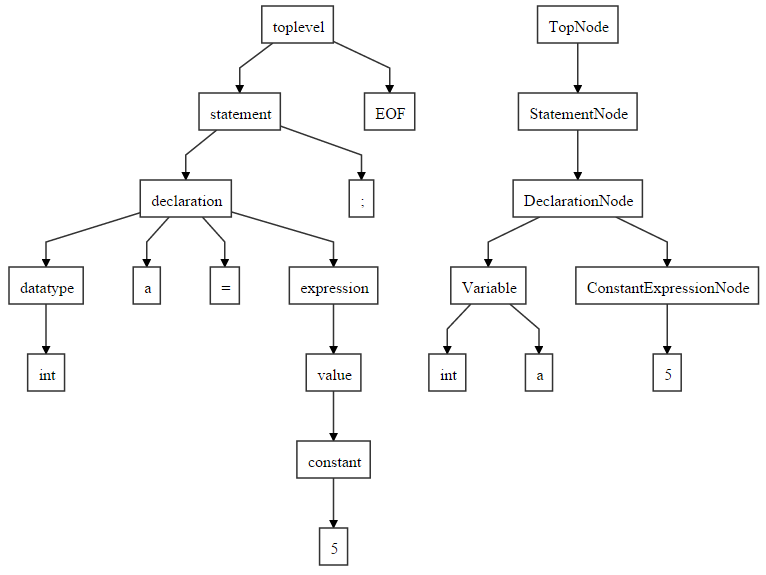
\includegraphics[width=0.8\linewidth]{figures/Trees/AST.PNG}
		\caption{The tree on the left is the parse tree, and the tree on the right is the AST, which still contains all the information from the parse tree.} \label{image:AST}
\end{figure}

As mentioned the parse tree is generated using a parser produced by compiling the grammar with ANTLR, which means we cannot decide what information is contained on the nodes of the tree.
The nodes of the \acrshort{ast} can therefore be made to contain information for type and scope checking, which makes those phases a lot easier.
All that is needed to make this transformation, is to make classes for all the nodes of the \acrshort{ast}, and create a way to traverse the AST.
The next section will present ways of traversing trees, while performing different computations like scope and type checking on the trees.


